\chapter{Succesive-Shortest-Path-Algorithmus}
Im folgenden Kapitel wird ein Blick auf einen weiteren Algorithmus geworfen, der verwendet werden kann, um einen kostenminimalen Fluss zu erzeugen.
\section{Einleitung}
Der Successive-Shortest-Path-Algorithmus (im folgenden SSPA) verwendet einen anderen Ansatz als der Cycle-Cancelling-Algorithmus. Der Cycle-Cancelling-Algorithmus benötigt als Input einen Graphen in dem ein $b$-Fluss möglich ist. Nachdem dieser berechnet ist spielt die Balance keine Rolle mehr. Denn sofern ein $b$-Fluss existiert muss immer eine Balance existieren. %ist das wirklich so?
Im Successive Shortest Path wird zunächst nicht auf den $b$-Fluss geschaut. Stattdessen wird darauf abgezielt solange günstige Wege zu finden bis alle Knoten ausbalanciert sind.

\section{Formaler Aufbau}
\begin{table}[H]
    \setlength{\tabcolsep}{20pt}
    \centering
    \begin{tabular}{p{2.5cm} >{\setstretch{1.5}}p{10cm}}
    \toprule
    \multicolumn{2}{l}{\textbf{Successive-Shortest-Path-Algorithmus}} \\ \midrule
    %\onehalfspacing
    Input:          & Gerichteter Graph $G = (V, E)$, obere Kapazitäten $u$, Kantenkosten $c$, Balance $b$.         \\
     ~ & ~ \\
    Output:         & Kostenminimaler Fluss $f$, falls existent, oder Aussage, dass keiner existiert.                \\
     ~ & ~ \\
    Schritt 1:      & Setzen Sie
       \[ f(e) = \begin{cases}
         0 & \text{falls } c(e) \ge 0 \\
         u(e) & \text{falls } c(e) < 0 
       \end{cases} \]
    und
    \begin{equation*}
        b'(v) = \displaystyle\sum_{e \in \delta ^{+} (v)}^{} f(e) - \displaystyle\sum_{e \in \delta ^{-} (v)}^{} f(e).
    \end{equation*}\\
    Schritt 2:      & Wählen Sie einen Knoten $s$ mit $b(s) - b'(s) > 0$ als Quelle und einen Knoten $t$ mit $b(t) - b'(t) < 0$ als Senke. Der Knoten $t$ muss vom Knoten $s$ im Residualgraph $G^f$ erreichbar sein. Dann gehen Sie zu Schritt 3. Existiert kein solches Paar aus $s$ und $t$ und $b(v) = b'(v)$ gilt für alle $v \in V$, dann ist $f$ kostenminimal. Ansonsten gibt es keinen $b$-Fluss.              \\
     ~ & ~ \\
    Schritt 3:      & Berechnen Sie einen kürzesten Weg $p$ bzgl. $c^f$ in $G^f$.               \\
     ~ & ~ \\
    Schritt 4:      & Verändern Sie den $b$-Fluss entlang des Weges p um den minimalen Wert aus Kapazität, Quelle und Senke:
    \begin{equation*}
        \gamma := min\{\underset{e \in p}{min} \{u^f (e) \}, b(s) - b'(s), b'(t) - b(t)\}.
    \end{equation*}              \\
     Schritt 5:     & Gehen Sie zu Schritt 2.              \\
                    &              \\ \bottomrule  
    \end{tabular}
\caption{Formaler Ablauf Successive-Shortest-Path}
\label{tab:form_sspa}
\end{table}
    
Um den Algorithmus wie er in der Tabelle \ref{tab:form_sspa} dargestellt ist, etwas greifbarer zu machen wird das zu Beginn erwähnte Logistikproblem herangezogen. Die Logistikzentren agieren als Quellen während die Verkaufsstandorte als Senken agieren. Die verschiedenen Routen haben entsprechende Kosten und Kapazitäten. 

\textbf{Schritt 1:} Der SSPA beginnt in Schritt 1 damit, den kostengünstigsten Weg darzustellen. Dazu maximiert er die Flüsse an den Stellen, an denen negative Kosten vorliegen (im Logistikbeispiel könnten damit bspw. andere Waren mitgenommen werden). Alle anderen Flüsse werden hingegen mit $0$ inititalisiert. Des Weiteren erhält jeder Knoten $v$ einen zusätzlichen Balancewert $b'(v)$.

\textbf{Schritt 2:} Ab hier beginnt eine Iteration. In jeder Iteration wird eine Quelle und eine Senke aus den Knoten aus dem Graphen ausgewählt die die entsprechenden Bedingungen erfüllen. In dem Logistikbeispiel würde das wieder einem Verkaufsstandort und einem Logistikzentrum entsprechen. Wenn kein solches Paar existiert, muss anschließend geprüft werden ob jeder Verkaufsstandort und jedes Logistikzentrum ausbalanciert ist. Also ob $b(v) = b'(v)$ für alle $v \in V$ gilt. Ist dies der Fall wird jeder Verkaufsstandort mit minimalen Kosten von den Logistikzentren versorgt. Ist dies nicht der Fall, bedeutet das, dass es entweder ein zu großes Angebot, eine zu große Nachfrage oder ein zu kleines Netzwerk gab. In diesem Fall ist es nicht möglich einen $b$-Fluss und damit einen kostenminimalen Fluss zu bilden.

\textbf{Schritt 3:} Anschließend muss in dem Residualgraphen ein kürzester Weg gefunden werden. Dazu kann wieder der Moore-Bellman-Ford-Algorithmus verwendet. Durch die Initialisierung im ersten Schritt kann es zu keinen negativen Zykeln im Residualgraphen kommen, wodurch dies keine Abbruchbedingung darstellt. Es wird also ein kürzester Weg zwischen einem Verkaufsstandort und einem Logistikzentrum gesucht.

\textbf{Schritt 4:} Der Weg zwischen Verkaufsstandort und Logistikzentrum wird in diesem Schritt verbessert. Dazu wird der Fluss entsprechend verändert. Das ändernde Gamma ermittelt sich aus den drei Attributen: Kapazität, Angebot und Nachfrage. Es kann nicht mehr gesendet werden als zur Verfügung steht, es kann nicht mehr empfangen werden als möglich und die Kapazität ist beschränkt. Entsprechend wird das Minimum dieser Attribute zur Veränderung verwendet. Das Gamma wird auf die Quelle und den Fluss addiert und von der Senke abgezogen. Die anderen Knoten bleiben unberührt.

\textbf{Schritt 5:} Die Iteration ist beendet und es geht wieder mit Schritt 2 weiter. 

\section{Beispiel}
Um die Anwendung des Algorithmus zu sehen, wird im Folgenden ein Durchlauf an einem Beispiel gezeigt. Der dazu verwendete Graph wird in seiner Form in Abbildung \ref{fig:sspa_initial} dargestellt.

\begin{figure}[H]
\centering
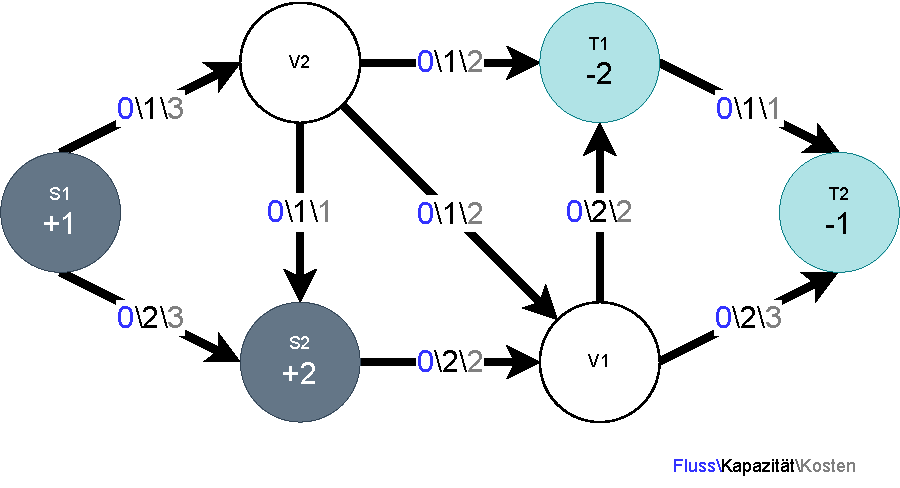
\includegraphics[width=0.8\textwidth]{img/anton/sspa-initial.pdf}
\caption{SSPA Initial}
\label{fig:sspa_initial}
\end{figure}

\begin{figure}[H]
\centering
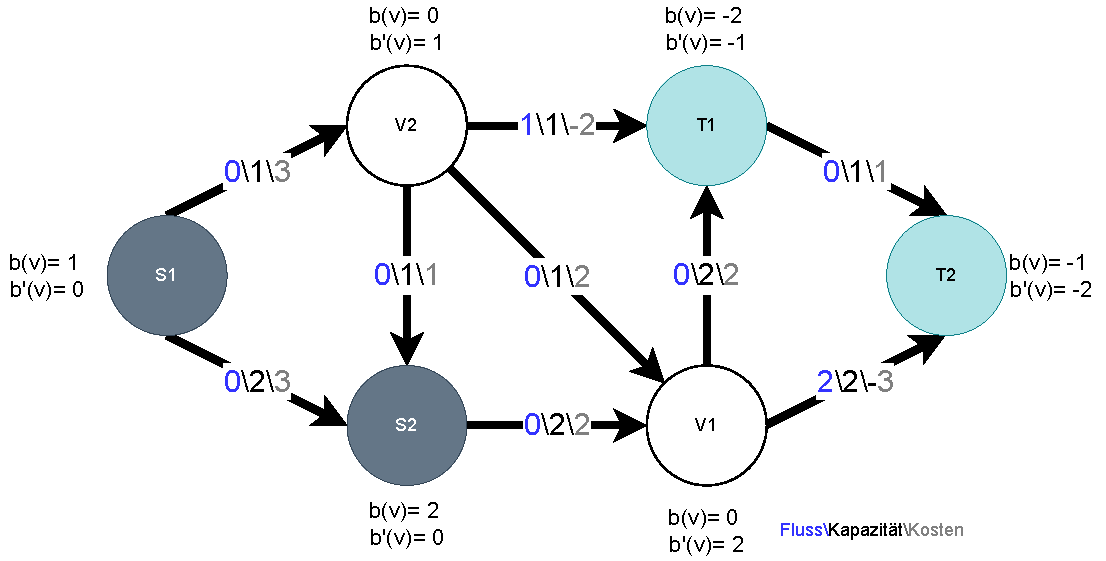
\includegraphics[width=0.9\textwidth]{img/anton/sspa-Step1.pdf}
\caption{SSPA Graph nach Schritt 1}
\label{fig:sspa_step1}
\end{figure}

In Abbildung \ref{fig:sspa_step1} ist der Graph nach Anwendung des ersten Schritts zu sehen. Die negativen Kanten sind maximiert, die restlichen Kanten auf $0$ gesetzt und jeder Knoten hat zu seiner Ziel-Balance $b(v)$ noch eine aktuelle Balance $b'(v)$ erhalten. Danach beginnt die erste Iteration.

\begin{figure}[H]
\centering
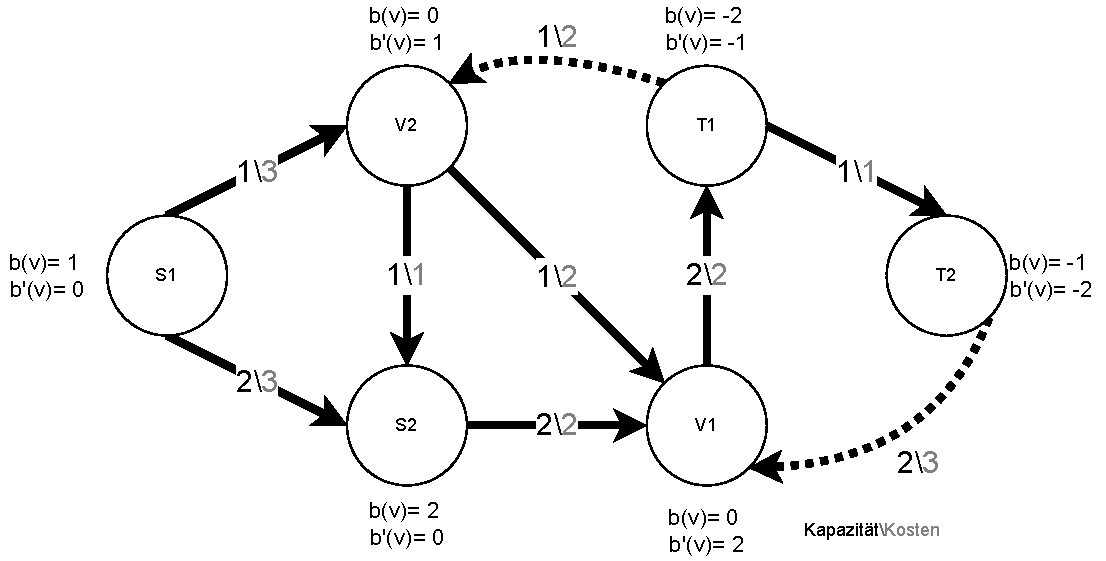
\includegraphics[width=0.9\textwidth]{img/anton/sspa-Step1-residual.pdf}
\caption{SSPA Iteration 1 Residualgraph}
\label{fig:sspa_step1-residual}
\end{figure}
%Reihenfolge noch anpassen?
Da es noch Quellen und Senken gibt, kann nun der Residualgraph aufgestellt werden um einen kürzesten Weg zwischen diesen zu finden. Dieser ist in Abbildung \ref{fig:sspa_step1-residual} zu sehen.

\begin{figure}[H]
\centering
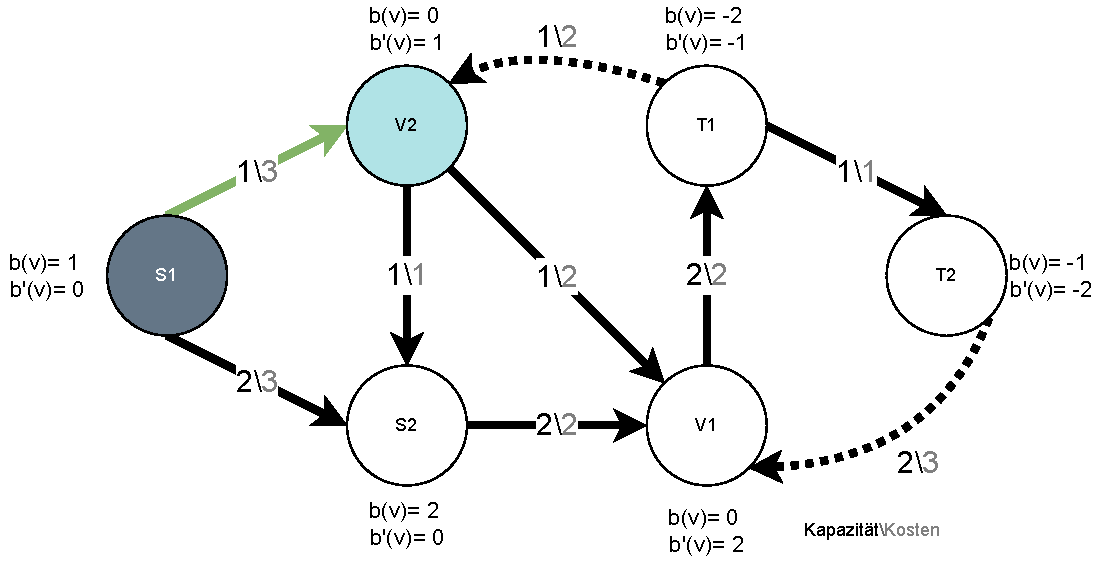
\includegraphics[width=0.9\textwidth]{img/anton/sspa-Step1-shortestPath.pdf}
\caption{SSPA Weg von $S1$ zu $V2$}
\label{fig:sspa_step1-shortestPath}
\end{figure}

In dem Beispiel wurde der Knoten $S1$ als Quelle und $V2$ als Senke verwendet (vgl. Abbildung \ref{fig:sspa_step1-shortestPath}. Nun kann mithilfe bspw. des Moore-Bellman-Ford-Algorithmus' ein kürzester Weg zueinander berechnet werden. Das Ergebnis davon ist hier grün eingezeichnet. Da ein kürzester Weg gefunden wurde, findet anschließend die Veränderung des Weges entlang des Flusses statt. Die Veränderung berechnet sich aus $\gamma := min\{\underset{e \in p}{min} \{u^f (e) \}, b(s) - b'(s), b'(t) - b(t)\} $, also $\gamma := min\{1, 1, 1\}$. In diesem Fall beträgt jeder der drei Werte $1$. An der Quelle und im Fluss finden daher eine Veränderung um $+1$ statt, während die Senke $-1$ erhält. Damit ist die erste Iteration beendet.

\begin{figure}[H]
\centering
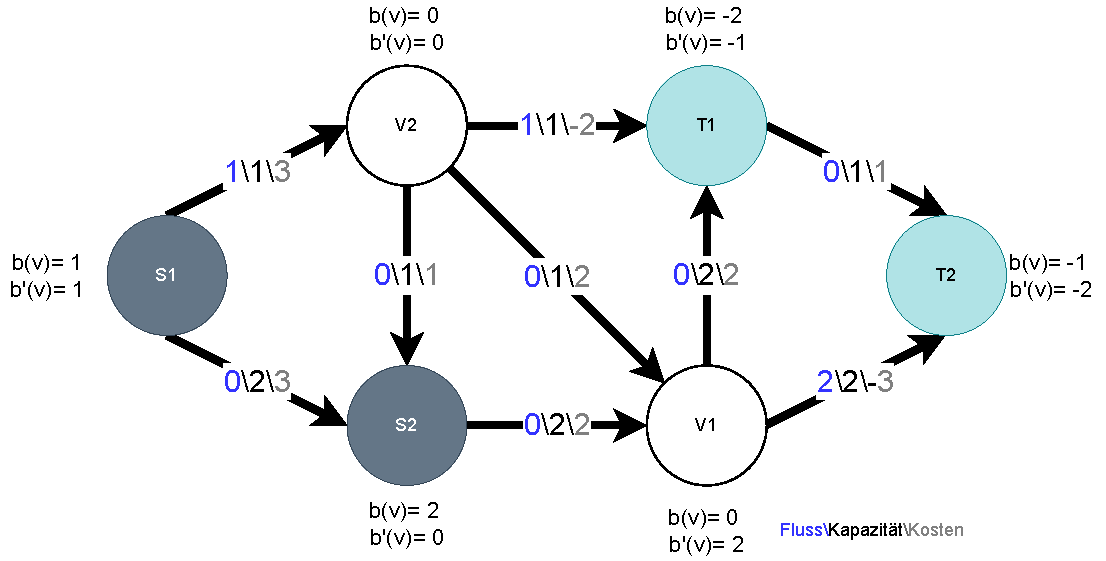
\includegraphics[width=0.9\textwidth]{img/anton/sspa-Step1-newGraph.pdf}
\caption{SSPA Graph nach Iteration 1}
\label{fig:sspa_step1-new-Graph}
\end{figure}

In Abbildung \ref{fig:sspa_step1-new-Graph} ist nun der Graph nach der ersten Iteration zu sehen. Anschließend beginnt die zweite Iteration.

\begin{figure}[H]
\centering
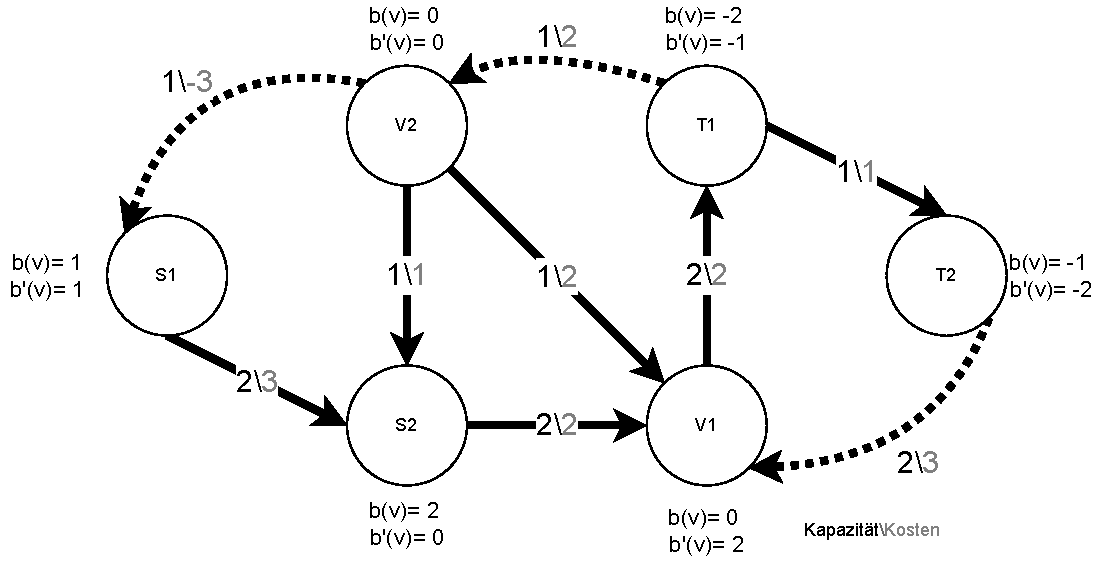
\includegraphics[width=0.9\textwidth]{img/anton/sspa-Step2-residual.pdf}
\caption{SSPA Iteration 2 Residualgraph}
\label{fig:sspa_step2-residual}
\end{figure}

Da es immer noch Quellen und Senken gibt, wird zu Beginn der zweiten Iteration erneut der Residualgraph gebildet (vgl. Abbildung \ref{fig:sspa_step2-residual}).

\begin{figure}[H]
\centering
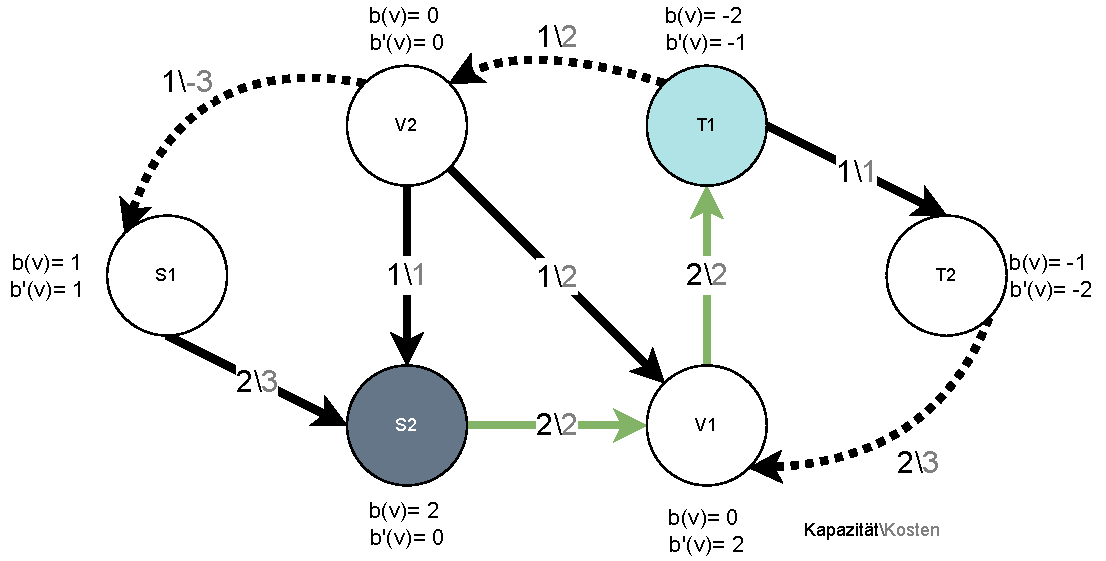
\includegraphics[width=0.9\textwidth]{img/anton/sspa-Step2-shortestPath.pdf}
\caption{SSPA Weg von $S2$ zu $T1$}
\label{fig:sspa_step2-shortestPath}
\end{figure}

\begin{figure}[H]
\centering
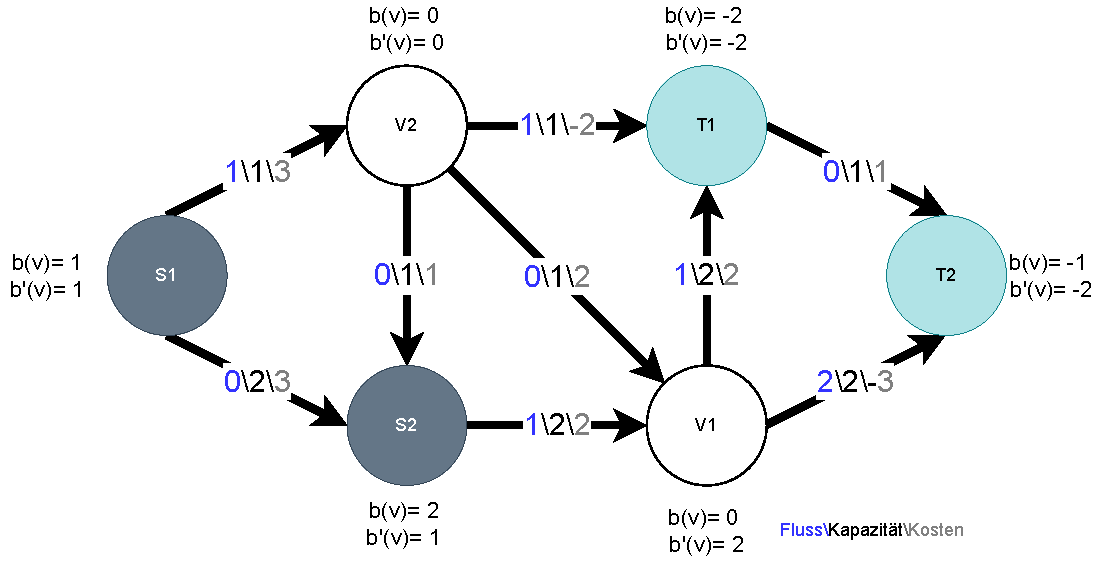
\includegraphics[width=0.9\textwidth]{img/anton/sspa-Step2-newGraph.pdf}
\caption{SSPA Graph nach Iteration 2}
\label{fig:sspa_step2-new-Graph}
\end{figure}

Anschließend wird erneut der kürzeste Weg zwischen Quelle und Senke gesucht (vgl. Abbildung \ref{fig:sspa_step2-shortestPath}). Das entstehende Gamma aus dem Weg von $S2$ zu $T1$ lautet $\gamma := min\{2, 2, 1\}$. Der Weg wird demnach erneut um den Wert $1$ verändert, wodurch der Graph aus Abbildung \ref{fig:sspa_step2-new-Graph} entsteht. Daraufhin startet die dritte Iteration mit dem Residualgraphen in Abbildung \ref{fig:sspa_step3-residual}.

\begin{figure}[H]
\centering
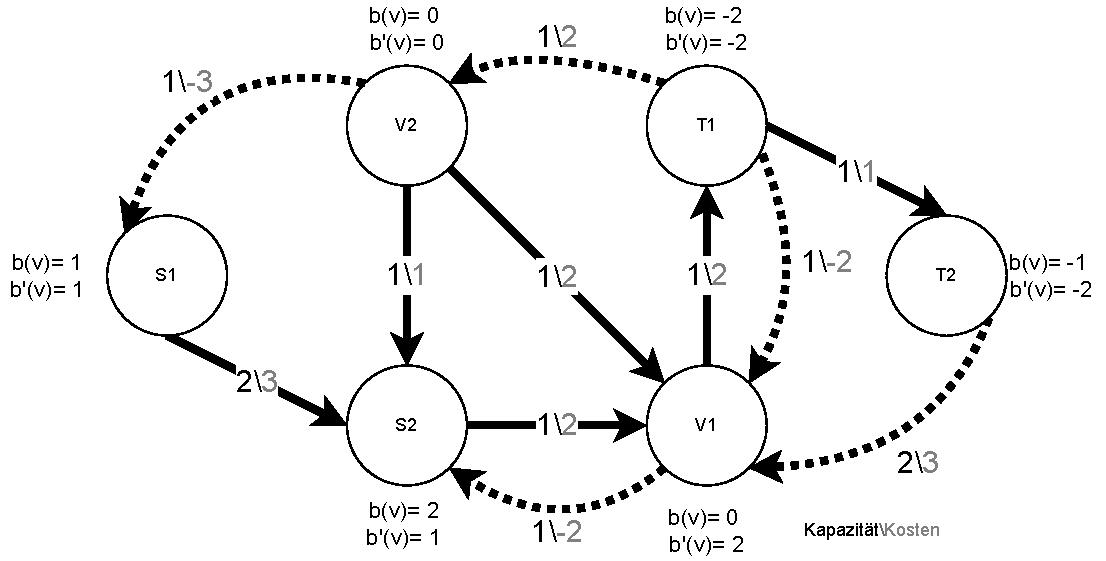
\includegraphics[width=0.9\textwidth]{img/anton/sspa-Step3-residual.pdf}
\caption{SSPA Iteration 3 Residualgraph}
\label{fig:sspa_step3-residual}
\end{figure}

\begin{figure}[H]
\centering
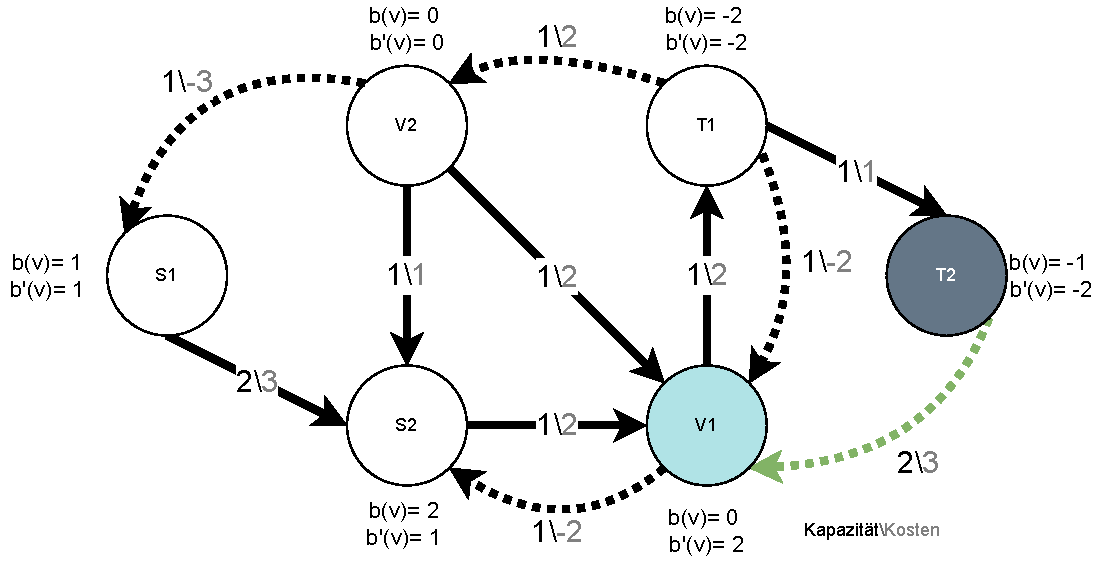
\includegraphics[width=0.9\textwidth]{img/anton/sspa-Step3-shortestPath.pdf}
\caption{SSPA Weg von $T2$ zu $V1$}
\label{fig:sspa_step3-shortestPath}
\end{figure}

In dem Graphen befinden sich noch zwei Quellen mit $S2$ und $T2$ und eine Senke mit $V1$. Es wird der Weg von $T2$ zu $V1$ mit dem entsprechenden kürzesten Weg gesucht (vgl. Abbildung \ref{fig:sspa_step3-shortestPath}. Das entstehende Gamma lautet: $\gamma := min\{2, 2, 1\}$, also 1. Nach der Veränderung entlang des Weges entsteht der Graph aus Abbildung \ref{fig:sspa_step3-new-Graph}.

\begin{figure}[H]
\centering
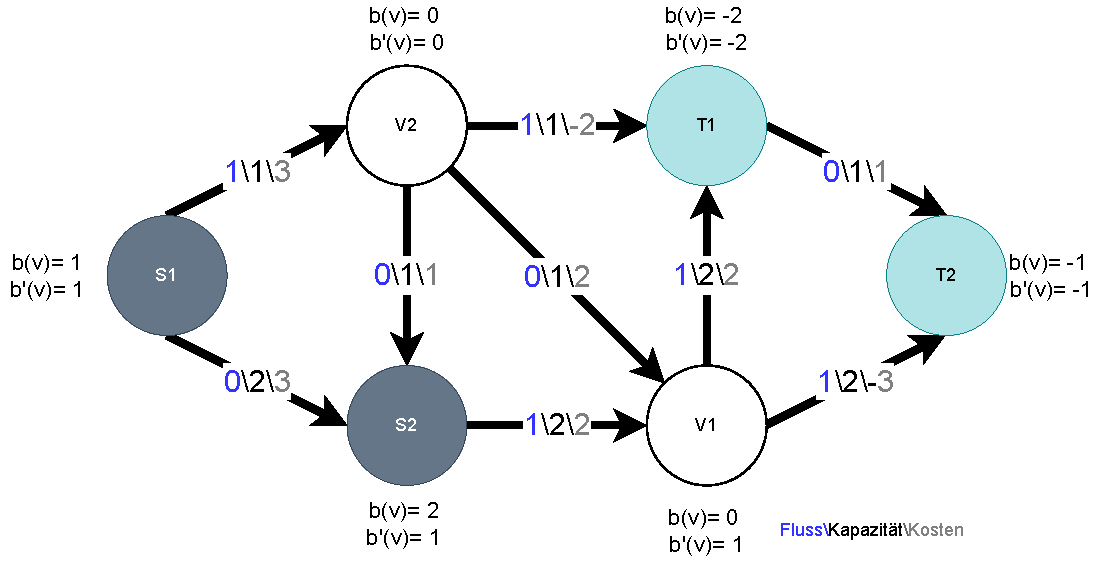
\includegraphics[width=0.9\textwidth]{img/anton/sspa-Step3-newGraph.pdf}
\caption{SSPA Graph nach Iteration 3}
\label{fig:sspa_step3-new-Graph}
\end{figure}

Aus dem Graphen geht es in die vierte Iteration mit dem Residualgraphen in Abbildung \ref{fig:sspa_step4-residual} und den verbleibenden Knoten $S2$ und $V1$, zwischen denen auch ein kürzester Weg mit $\gamma := min\{1, 1, 1\}$ gefunden werden kann (vgl. Abbildung \ref{fig:sspa_step4-shortest-Path}. Nachdem die Veränderung entlang des Weges abgeschlossen ist, entsteht der Graph aus Abbildung \ref{fig:sspa_step4-new-Graph}.

\begin{figure}[H]
\centering
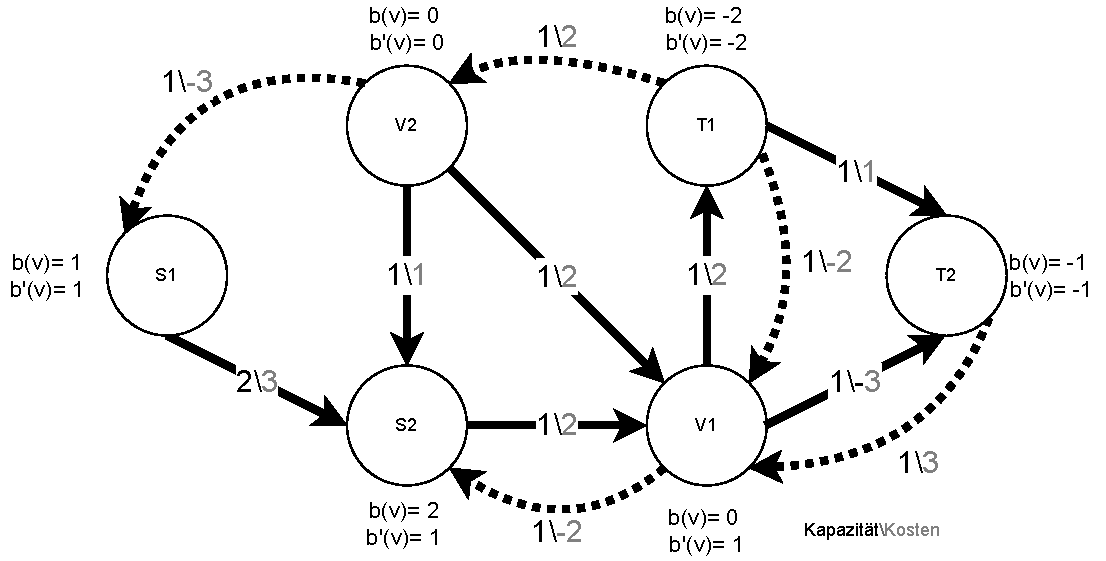
\includegraphics[width=0.9\textwidth]{img/anton/sspa-Step4-residual.pdf}
\caption{SSPA Iteration 4 Residualgraph}
\label{fig:sspa_step4-residual}
\end{figure}

\begin{figure}[H]
\centering
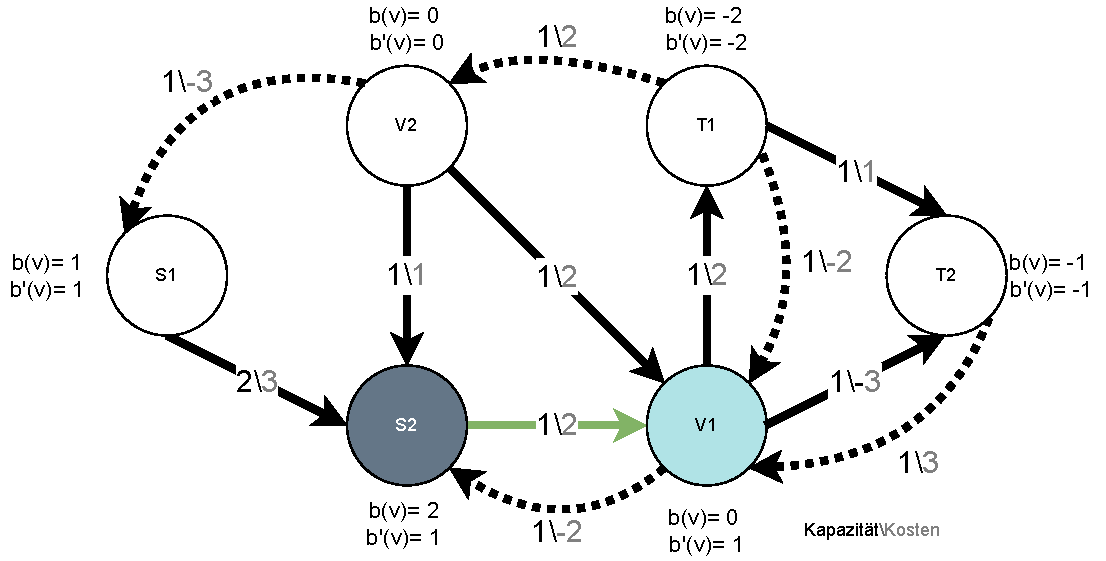
\includegraphics[width=0.9\textwidth]{img/anton/sspa-Step4-shortestPath.pdf}
\caption{SSPA Weg von $S2$ nach $V1$}
\label{fig:sspa_step4-shortest-Path}
\end{figure}

\begin{figure}[H]
\centering
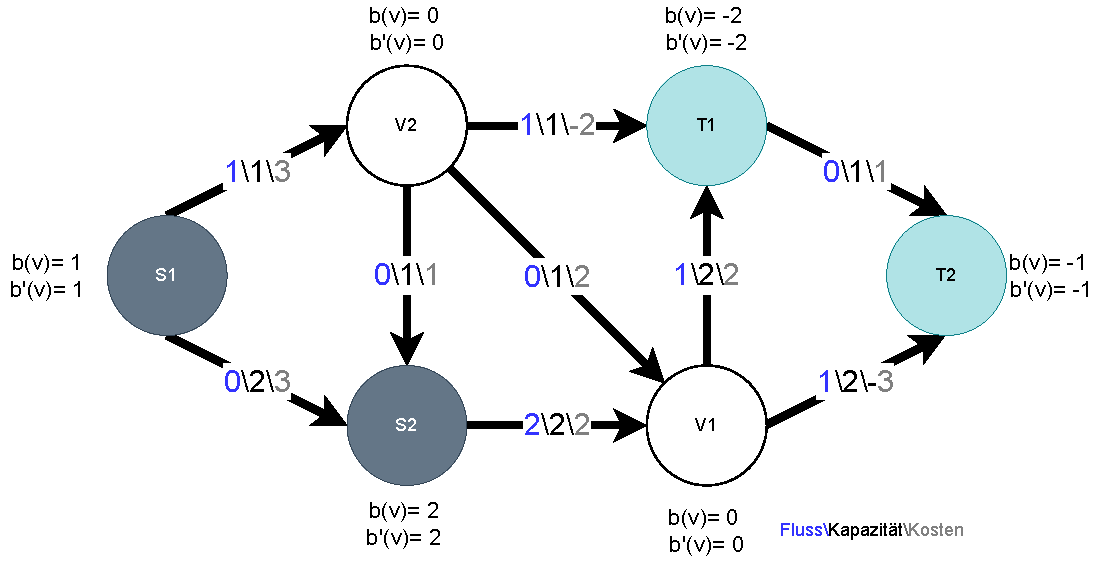
\includegraphics[width=0.9\textwidth]{img/anton/sspa-Step4-newGraph.pdf}
\caption{SSPA Graph nach Iteration 4}
\label{fig:sspa_step4-new-Graph}
\end{figure}

Da es keine Quellen und keine Senken mehr gibt, muss nun geprüft werden ob für alle Knoten $b(v) = b'(v)$ gilt. Da dies der Fall ist, findet sich der finale Graph mit den entstandenen Flusswerten in Abbildung \ref{fig:sspa_step5-final}.

\begin{figure}[H]
\centering
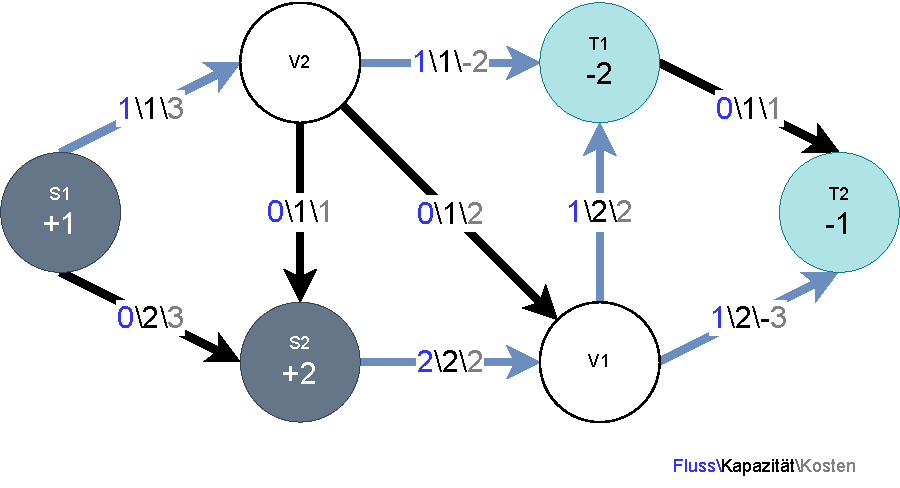
\includegraphics[width=0.8\textwidth]{img/anton/sspa-Step5-FinalMitFluss.pdf}
\caption{SSPA finaler Graph mit kostenminimalem $b$-Fluss}
\label{fig:sspa_step5-final}
\end{figure}

Um den finalen Wert zu errechnen muss nun die Formel aus Definition \ref{def:costfunktion} angewendet werden. Nach der Betrachtung aller Kanten ergeben sich die finalen Kosten von $4$.

\section{Fazit}
Der SSPA ist ein Weg um immer einen Kostenminimalen Fluss zu finden sofern er existiert. Des Weiteren darf im Verlauf des Algorithmus kein negativer Zykel auftreten, da dann der Moore-Bellmann-Ford-Algorithmus nicht mehr funktionieren würde. Zudem muss bei der Verwendung von ungerichteten Graphen darauf geachtet werden wie die Kanten aufgestellt werden. Weitere Informationen dazu finden sich bei \cite{sspa}. Die Komplexität des Algorithmus beträgt laut \cite{sspa} $O(n^2m^2)$ wobei es sich aus $O(nm) * T(n,m)$ zusammensetzt. Hierbei stellt T den Moore-Bellman-Ford-Algorithmus dar.